\documentclass{beamer}

\usepackage[utf8]{inputenc}
\usepackage{graphicx}
\usepackage{appendixnumberbeamer}

\usetheme{CambridgeUS}
\usecolortheme{beaver}

\setbeamertemplate{navigation symbols}{}

\title[ProbEmbed]{Learning Embeddings with Dirichlet Processes and Heavy Tails}
\author{Adith -- Chenhao -- Moontae}
\institute{Cornell}
\date{September 2014}

\begin{document}
\begin{frame}
\titlepage
\end{frame}

\begin{frame}{Learning embeddings}
  \begin{itemize}
    \item Mapping discrete atoms (words/phrases) into a continuous space
    \item Useful representation for several NLP tasks \cite{Turian}
  \end{itemize}
\begin{figure}[h!]
  \caption{Discovering implicit relationships between words \cite{CBOW}}
  \centering
    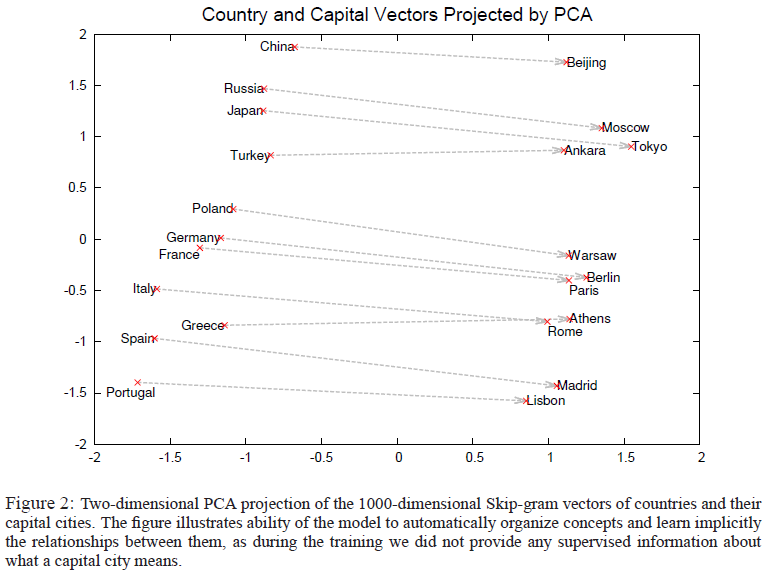
\includegraphics[width=0.5\textwidth]{CBOW.png}
\end{figure}
\end{frame}

\begin{frame}{An incomplete and utter history of word embeddings}
\begin{tabular}{p{0.5\textwidth}p{0.5\textwidth}}
 \begin{minipage}{.48\textwidth}
  \begin{itemize}
    \item Distributional clustering \cite{Lillian}
    \item SENNA \cite{Collobert}
    \item WordReprs \cite{Turian}
    \item NCE \cite{Mnih}
    \item Multi-prototype \cite{Socher}
    \item CBOW/Skip-gram \cite{CBOW}
    \item Matrix factorization approaches \cite{Moitra}
    \item Generative Topic Models \cite{LDA}
  \end{itemize}
\end{minipage}
&
\begin{minipage}{.48\textwidth}
\begin{figure}[h!]
  \caption{Discovering concept clusters \cite{Socher}}
  \centering
    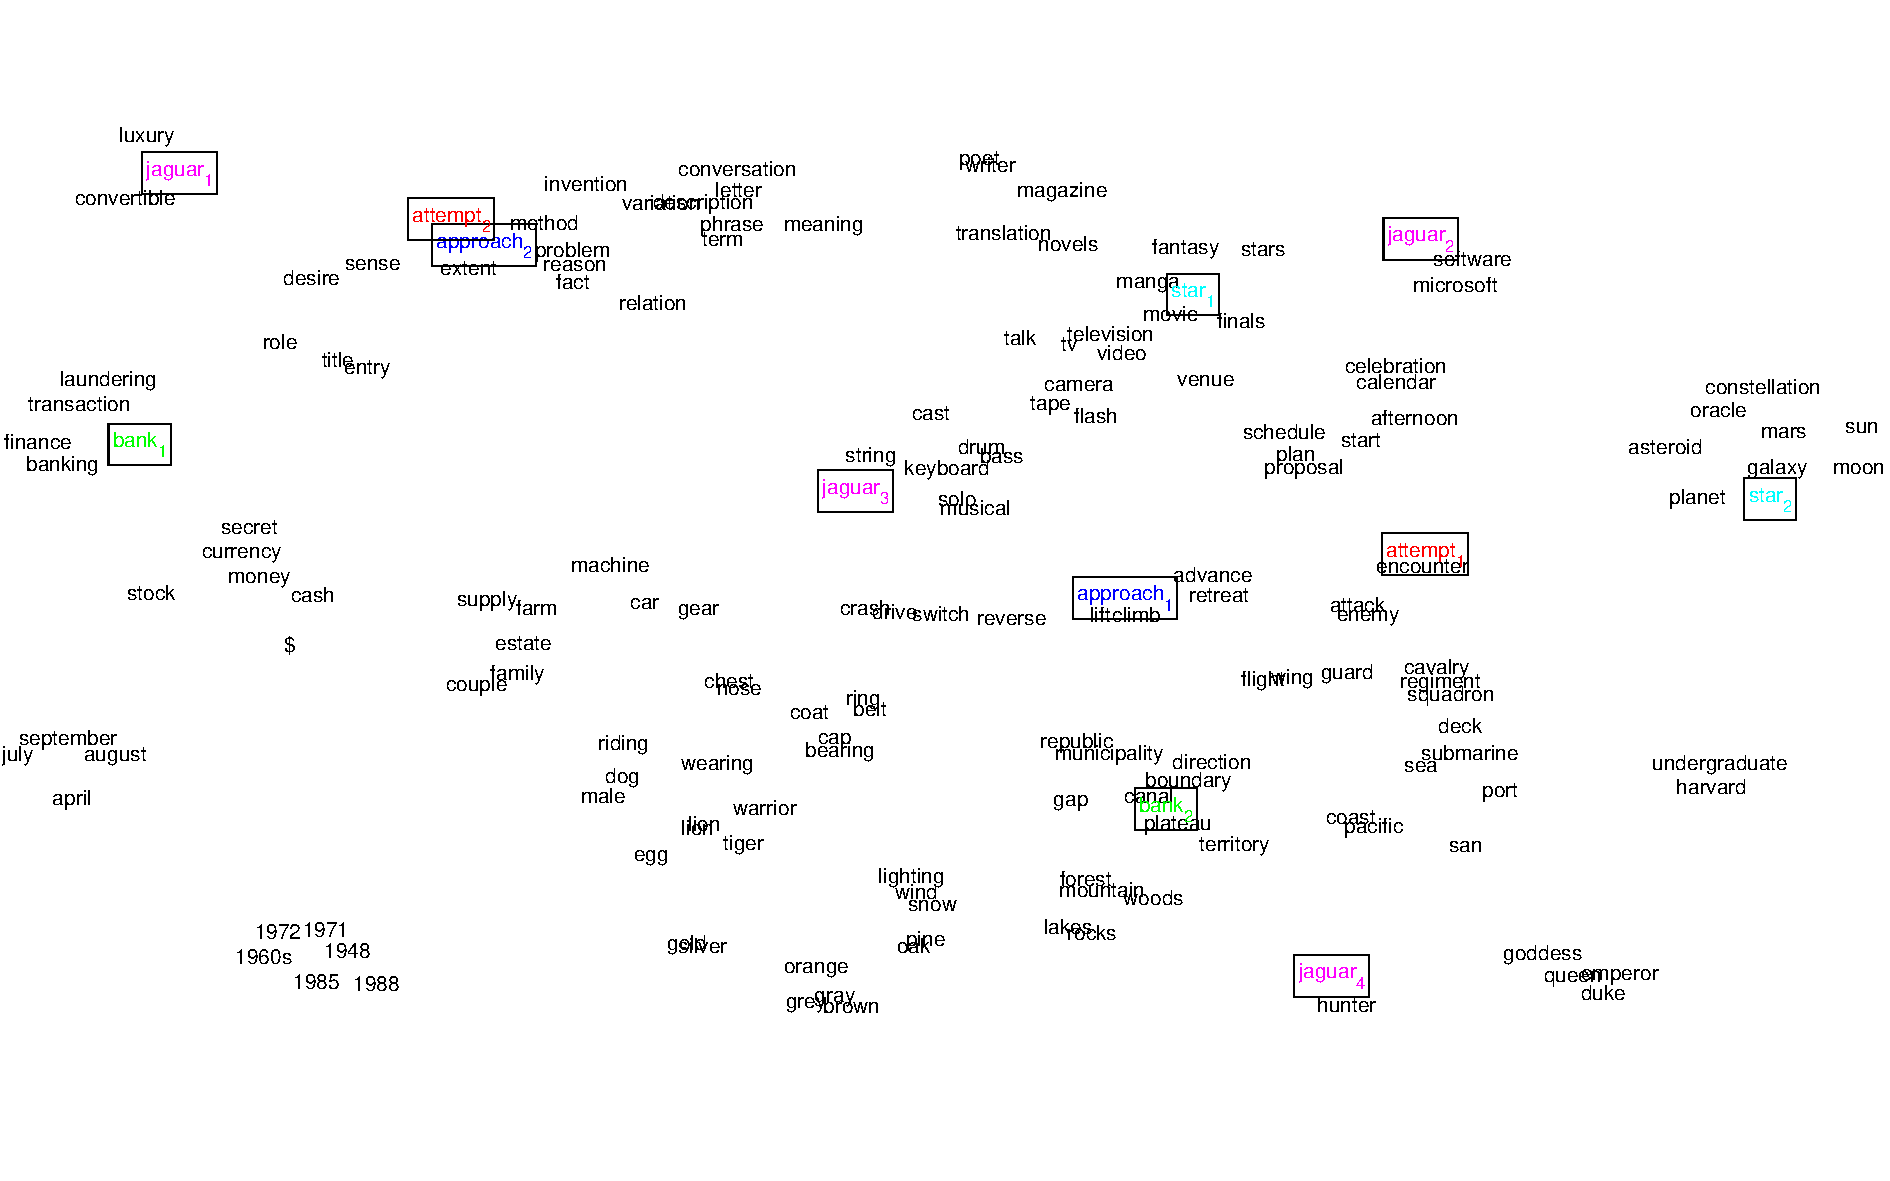
\includegraphics[width=0.9\textwidth]{MultipleVectorWordEmbedding.pdf}
\end{figure}
\end{minipage}
\end{tabular}
\end{frame}

\begin{frame}{Goal}
A generative model of word embeddings that
\begin{itemize}
\item Takes as input $D$: all observed text
\item Outputs an embedding $X$: words situated in a vector space
\item such that the embeddings cluster around concepts
\item distances/directions in the embedding space directly model data distribution
\item which is scalable to learn
\item and also recover good performance of existing embeddings in other settings
\end{itemize}
\end{frame}

\begin{frame}{Why generative models?}
  \begin{itemize}
    \item Learning problem is well specified
    \item Modular models for adding complexity/assumptions
    \item Embedding quality aligned with learning objective
    \item Diagnostics to verify model assumptions
  \end{itemize}
\end{frame}

\begin{frame}{Formal specification}
  \begin{block}{Bayesian framework}
    $\Pr(X)$: prior\\
    $\Pr(D \mid X)$: likelihood
  \end{block}
  \begin{block}{Learning problem}
	$X^* = argmax_{ X } \Pr(X \mid D) = argmax_{ X } \Pr(X) \cdot \Pr(D \mid X)$
  \end{block}
  \begin{block}{Evaluation}
	$\Pr(D_{heldout} \mid X^*)$\\
    Are ground-truth clusters preserved in embedding?\\
    etc.
  \end{block}
  \pause
  \begin{alertblock}{Question}
	What other evaluations should we do \& who to compare against?
  \end{alertblock}
\end{frame}

\begin{frame}{Example: Logistic Markov Embedding}
  \begin{block}{Embedding songs from playlists}
  	\begin{itemize}
    		\item $D: $ Playlists $p = s_1 \dots s_{|p|}$, first order markov chains
    		\item $s_i \mapsto X_i \overset{iid}{\sim} \mathcal{N}(\vec{0}, \lambda^2 \mathcal{I})$\\
    		\item $\Pr(s_j \mid s_i ; X) = \frac{exp(-\| X_i - X_j \|^2)}{\sum_{j'} exp(-\| X_i - X_{j'} \|^2)}$
    \end{itemize}
    \end{block}
    \begin{block}{Learning}
    		$argmax_{ X } \sum_p \sum_{i=1}^{|p|-1} \log \Pr(s_{i+1} \mid s_i ; X) + \sum_i \log \Pr(X_i) \equiv$\\
		$argmin_{ X } -\sum_i \sum_j \#(s_i \rightarrow s_j) \cdot \log \Pr(s_j \mid s_i ; X) + \frac{1}{2 \lambda^2} \sum_i \| X_i \|^2$
    \end{block}
\end{frame}

\begin{frame}{Logistic vs. Heavy-Tailed Dirichlet Process Markov Embedding}
\begin{columns}[c]
\column{5.5cm}
\begin{figure}
  \caption{Logistic Markov Embedding on \emph{YES-small} dataset \cite{LME}}
    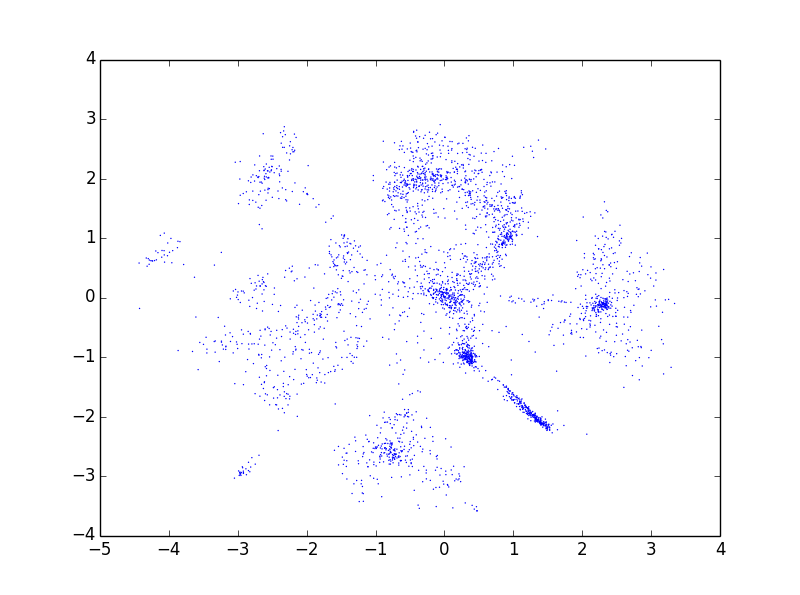
\includegraphics[width=0.9\textwidth]{LME.png}
\end{figure}
\column{5.5cm}
\pause
\begin{figure}
  \caption{Heavy-tailed Dirichlet Process Embedding}
    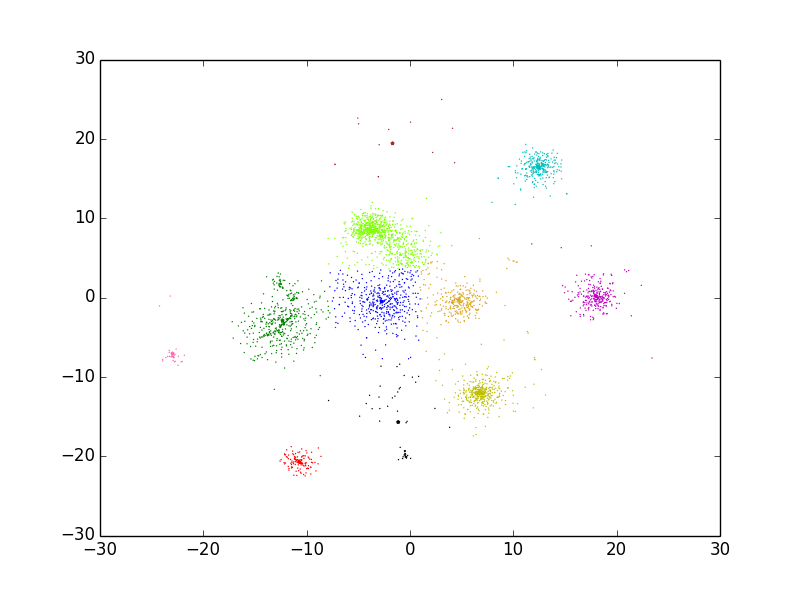
\includegraphics[width=0.9\textwidth]{ProbEmbed.png}
\end{figure}
\end{columns}
\end{frame}

\begin{frame}{Heavy-Tailed Dirichlet Process Markov Embedding}
  \begin{block}{DPMeans}
  Uses \cite{DPMeans}
   \end{block}

\end{frame}

\begin{frame}{Replacement game}
  \begin{block}{Model heavy tail distributions}
    $$Pr(w_j|w_i, X) = \frac{\frac{1}{1+(X_i-X_j)^2}}{\sum_{w}\frac{1}{1+(X_w-X_i)^2}}$$
  \end{block}
  \pause
  \begin{block}{Learning problem}
    $$argmin_{X, \mu, z, k} -\sum_{i}\sum_{j}Pr(w_j|w_i, X)+\lambda(\sum_i|||X_i-\mu_{z_i}|_2^2 + \sigma k)$$
  \end{block}
\end{frame}

\begin{frame}{Questions?}
  \begin{itemize}
    \item Replacement game, generation game or other likelihood?
    \item Can we actually evaluate based on generative story?
    \item What other evaluations should we do \& who to compare with?
  \end{itemize}
\end{frame}

\appendix

\begin{frame}[allowframebreaks]{References}
  \bibliographystyle{apalike}
  \bibliography{ProbEmbed}
\end{frame}

\end{document}